To make maximal use of the event information we have performed a multivariate analysis 
using a multivariate classifier based on the Boosted Decision Tree (BDT) technique. 
The BDT is implemented using the TMVA~\cite{tmva} toolkit and has been 
successfully applied in high energy physics to increase the 
statistical significance of a signal extraction
It requires less training than other multivariate classifiers and 
it is insensitive to the inclusion of poorly discriminating input variables.

In addition to the $\WW$ preselection, we apply a loose cut on the
maximum $\mll$ to enhance the signal-to-background ratio shown in Table~\ref{tab:presel_tmva_analysis}. 
The multivariate technique uses the following additional variables compared to the cut-based analysis: 
\begin{itemize}
\item $\Delta R_{\Lep\Lep}\equiv\sqrt{\deletall^2 + \delphill^2}$ between the leptons, 
with $\deletall$ the $\eta$ difference between the leptons, 
which has similar properties as $\delphill$
\item lepton flavors ($\mu\mu$, $ee$, $e\mu$ or $\mu e$ );
\item finally, for the 1-jet bin, the azimutal angles between the dilepton 
system and $\met$, and between the dilepton system and the 
highest $\pt$ jet, are included.
\end{itemize}

The training has been carried out separately in the 0-jet and 1-jet bins 
for different Higgs masses using the corresponding signal samples. For the background, 
we have considered $\WW$ processes only for now. The classifier outputs 
for three different Higgs masses and both jet bins are shown in 
Figures~\ref{fig:histo_mva_130}-\ref{fig:histo_mva_200}. 

The cut on the BDT output has been chosen to maximize 
the statistical significance $S$ defined as:
\begin{equation*}
S=\frac{N_S}{\sqrt{N_B+(\Delta N_B)^2}},
\end{equation*}
where $N_S$ and $N_B$ are the expected signal and background event yields, 
assuming the SM cross-sections and 1 $\ifb$ of integrated luminosity. 
Exclusively for the cuts optimization, the relative uncertainty 
$\Delta N_B/N_B$ on the combined background is considered to be equal to 35\%. 
This is just a rough estimation of the overall uncertainty. We have tested 
other values between 20\% and 50\% and obtained consistent results. It is 
worth mentioning that this method is not perfectly correct for cases with low 
number of events, and hence it is expected to see some small jumps in the 
signal and background yields for consecutive Higgs mass points. 
The expected number of signal and background events for an integrated luminosity 
of 1 $\ifb$, after applying the full multivariate analysis selection in the 0-jet and 1-jet 
bin cases are listed in Tables~\ref{tab:mvasel0j} and ~\ref{tab:mvasel1j}, respectively. 
The $gg \to H \to WW$ simulated events are reweighted to match the Higgs $\pt$ at NNLO, 
as explained in Section~\ref{sec:datasets}; all data-driven corrections are not applied.

\begin{table}
\begin{center}
\begin{tabular}{|r|c|c|c|c|c|c|c|c|c|c|c|c|}
\hline
$\mHi~~~~~[\GeV]$   & 120 & 130 & 140 & 150 & 160 & 170 & 180 & 190 & 200 & 210 \\
\hline
$\mll<~~~[\GeV]$    &  70 &  80 &  90 & 100 & 100 & 100 & 110 & 120 & 130 & 140 \\
\hline
\end{tabular}
%\vspace{0.5cm}
\begin{tabular}{|r|c|c|c|c|c|c|c|c|c|c|c|}
\hline
$\mHi~~~~~[\GeV]$    & 220 & 230 & 250 & 300 & 350 & 400 & 450 & 500 & 550 & 600 \\
\hline
$\mll<~~~[\GeV]$     & 150 & 230 & 250 & 300 & 350 & 400 & 450 & 500 & 550 & 600 \\
\hline
\end{tabular}
\caption{$\mll$ upper limit requirement as a function of the Higgs mass used to 
enrich the background datasets of signal-like events. These samples are employed 
in the training of the multivariate classifier used for the signal 
extraction.\label{tab:presel_tmva_analysis}}
\end{center}
\end{table}

\begin{figure}[!ht]
\begin{center}
   \subfigure[]{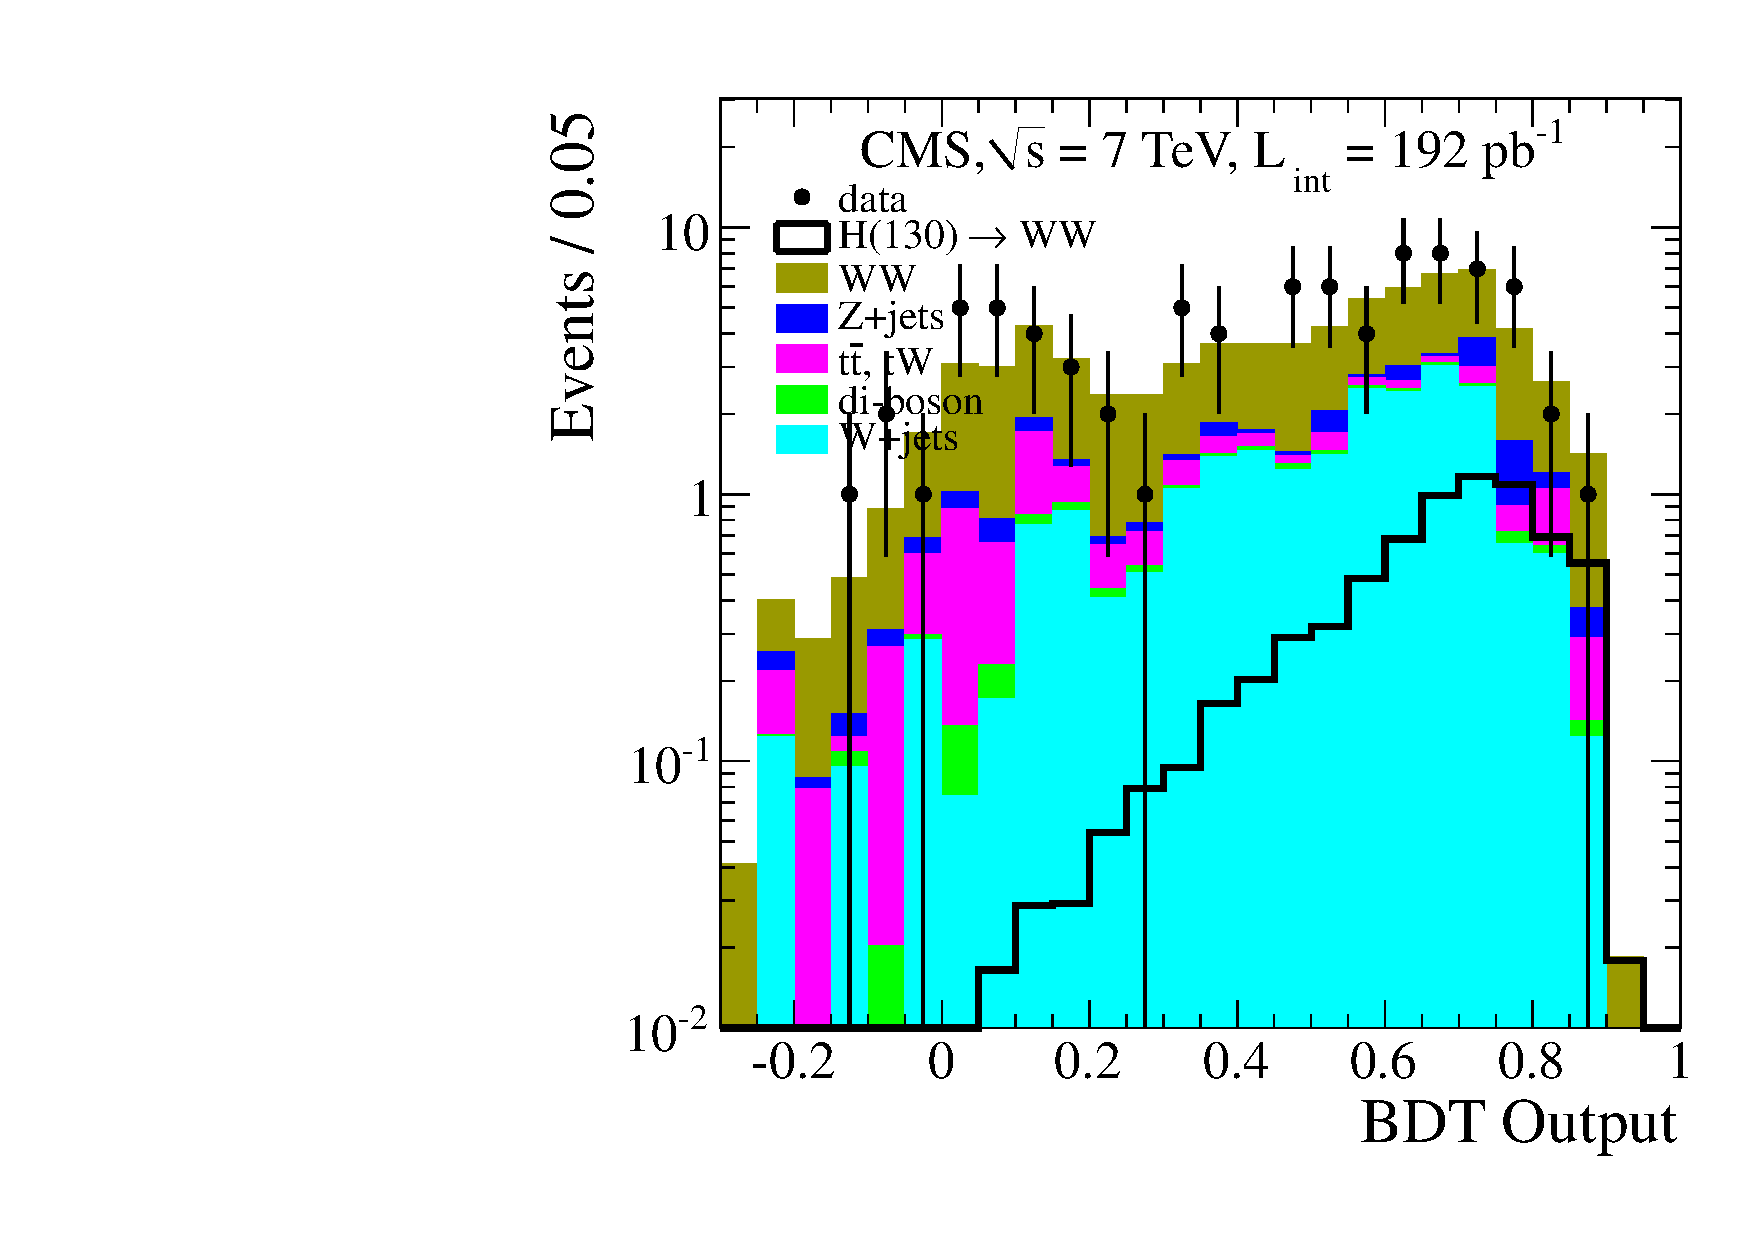
\includegraphics[width=0.49\textwidth,angle=0]{figures/histo_mva_130_0j.pdf}} 
   \subfigure[]{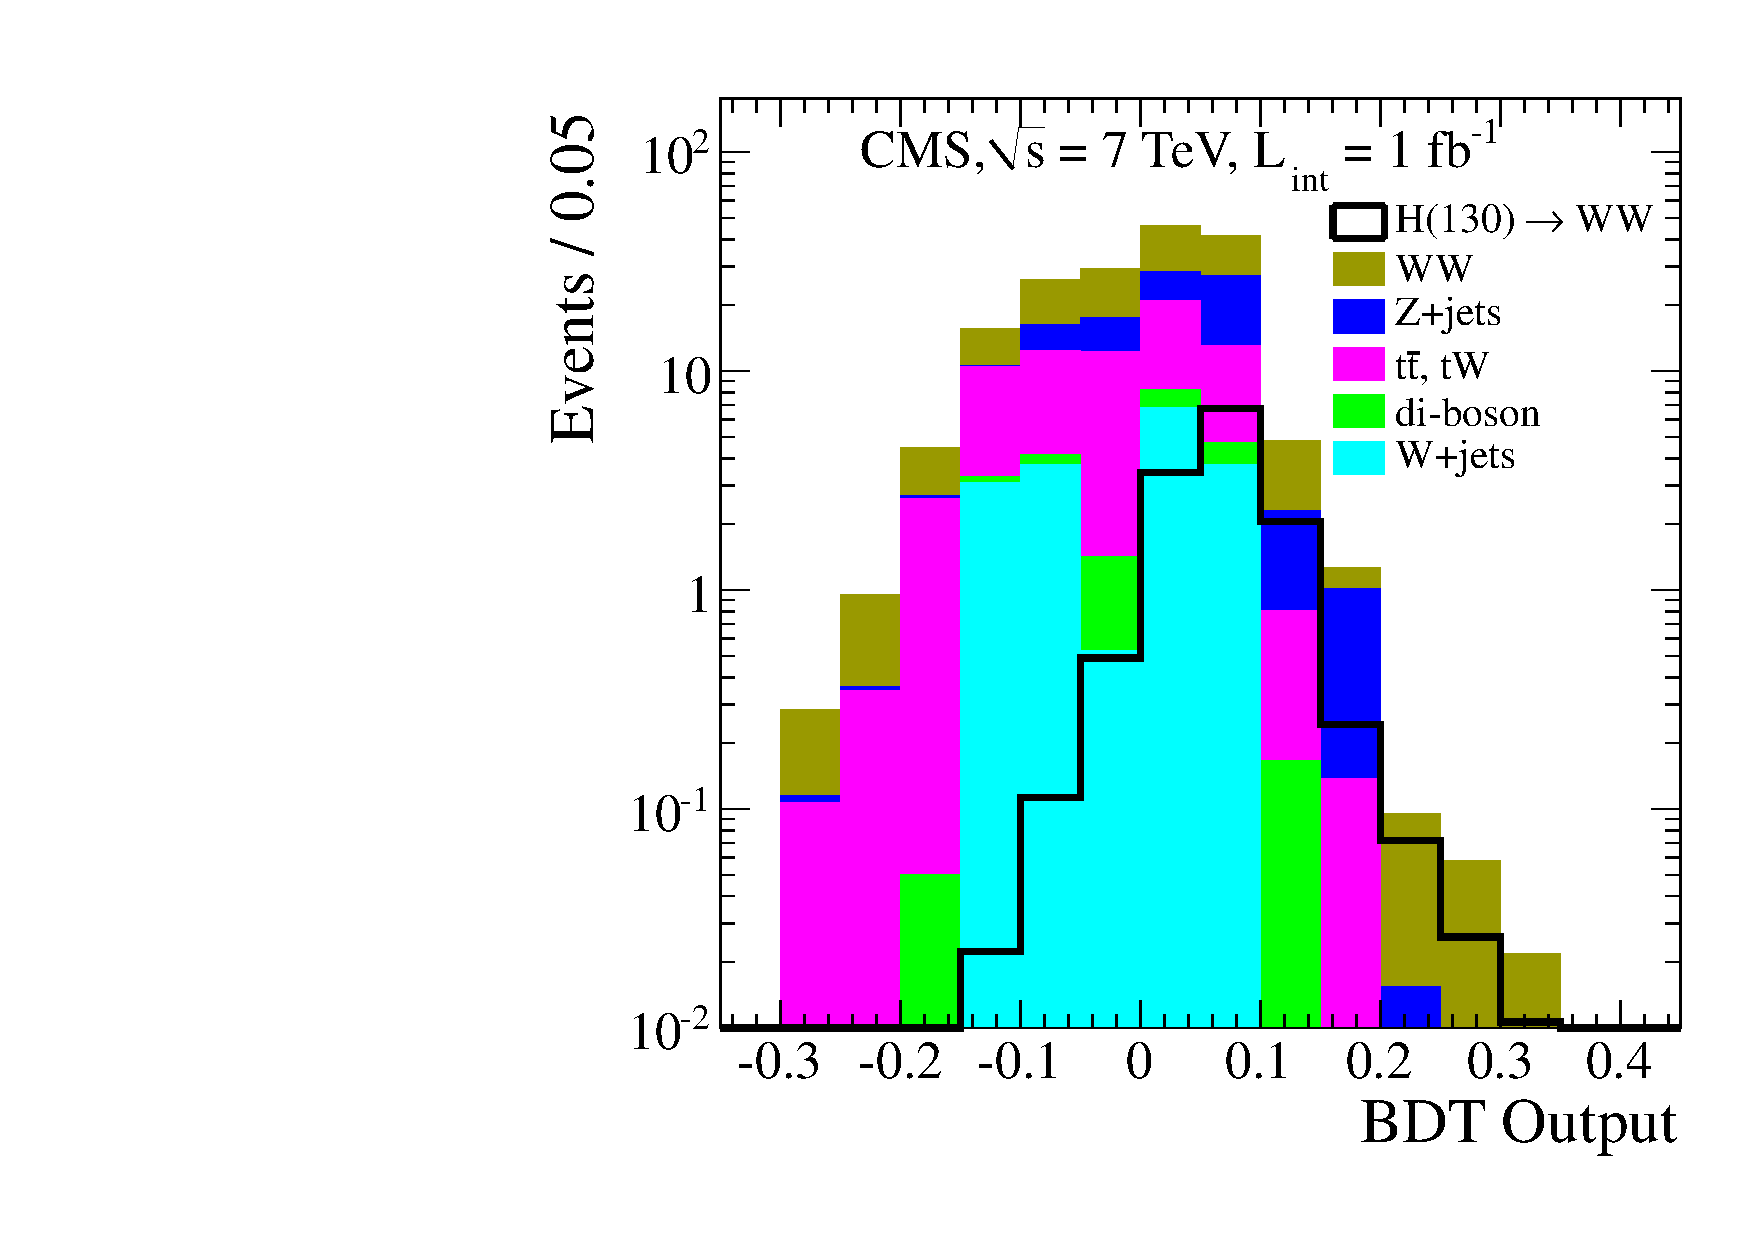
\includegraphics[width=0.49\textwidth,angle=0]{figures/histo_mva_130_1j.pdf}} 
       \caption{Classifier outputs for Higgs signal and background events 
for \mHi=130 $\GeVcc$ in the 0-jet bin (a) and 1-jet bin (b) after the $\WW$ selection. The number 
of events is different on each mass point due to the specific $\mll$ requirement.}
   \label{fig:histo_mva_130}
\end{center}
\end{figure}

\begin{figure}[!ht]
\begin{center}
   \subfigure[]{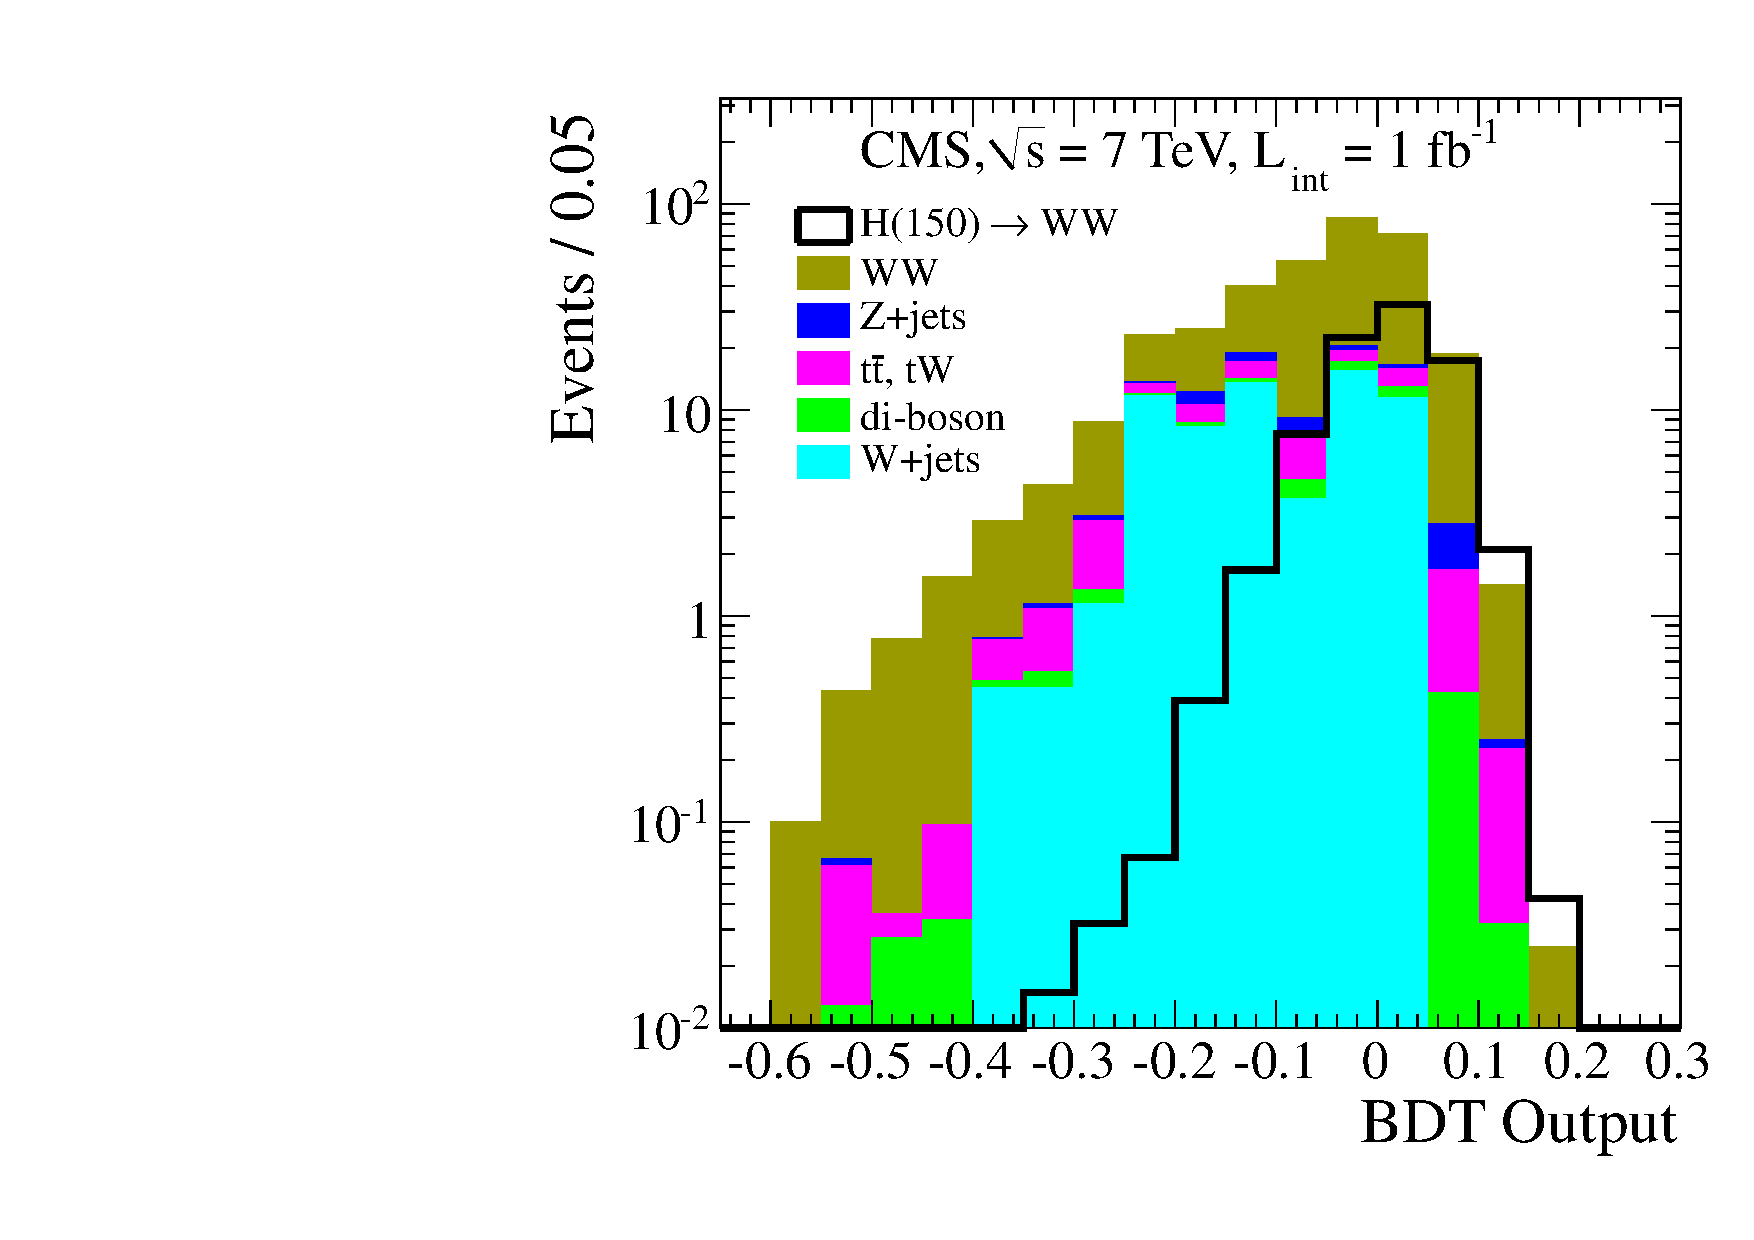
\includegraphics[width=0.49\textwidth,angle=0]{figures/histo_mva_150_0j.pdf}} 
   \subfigure[]{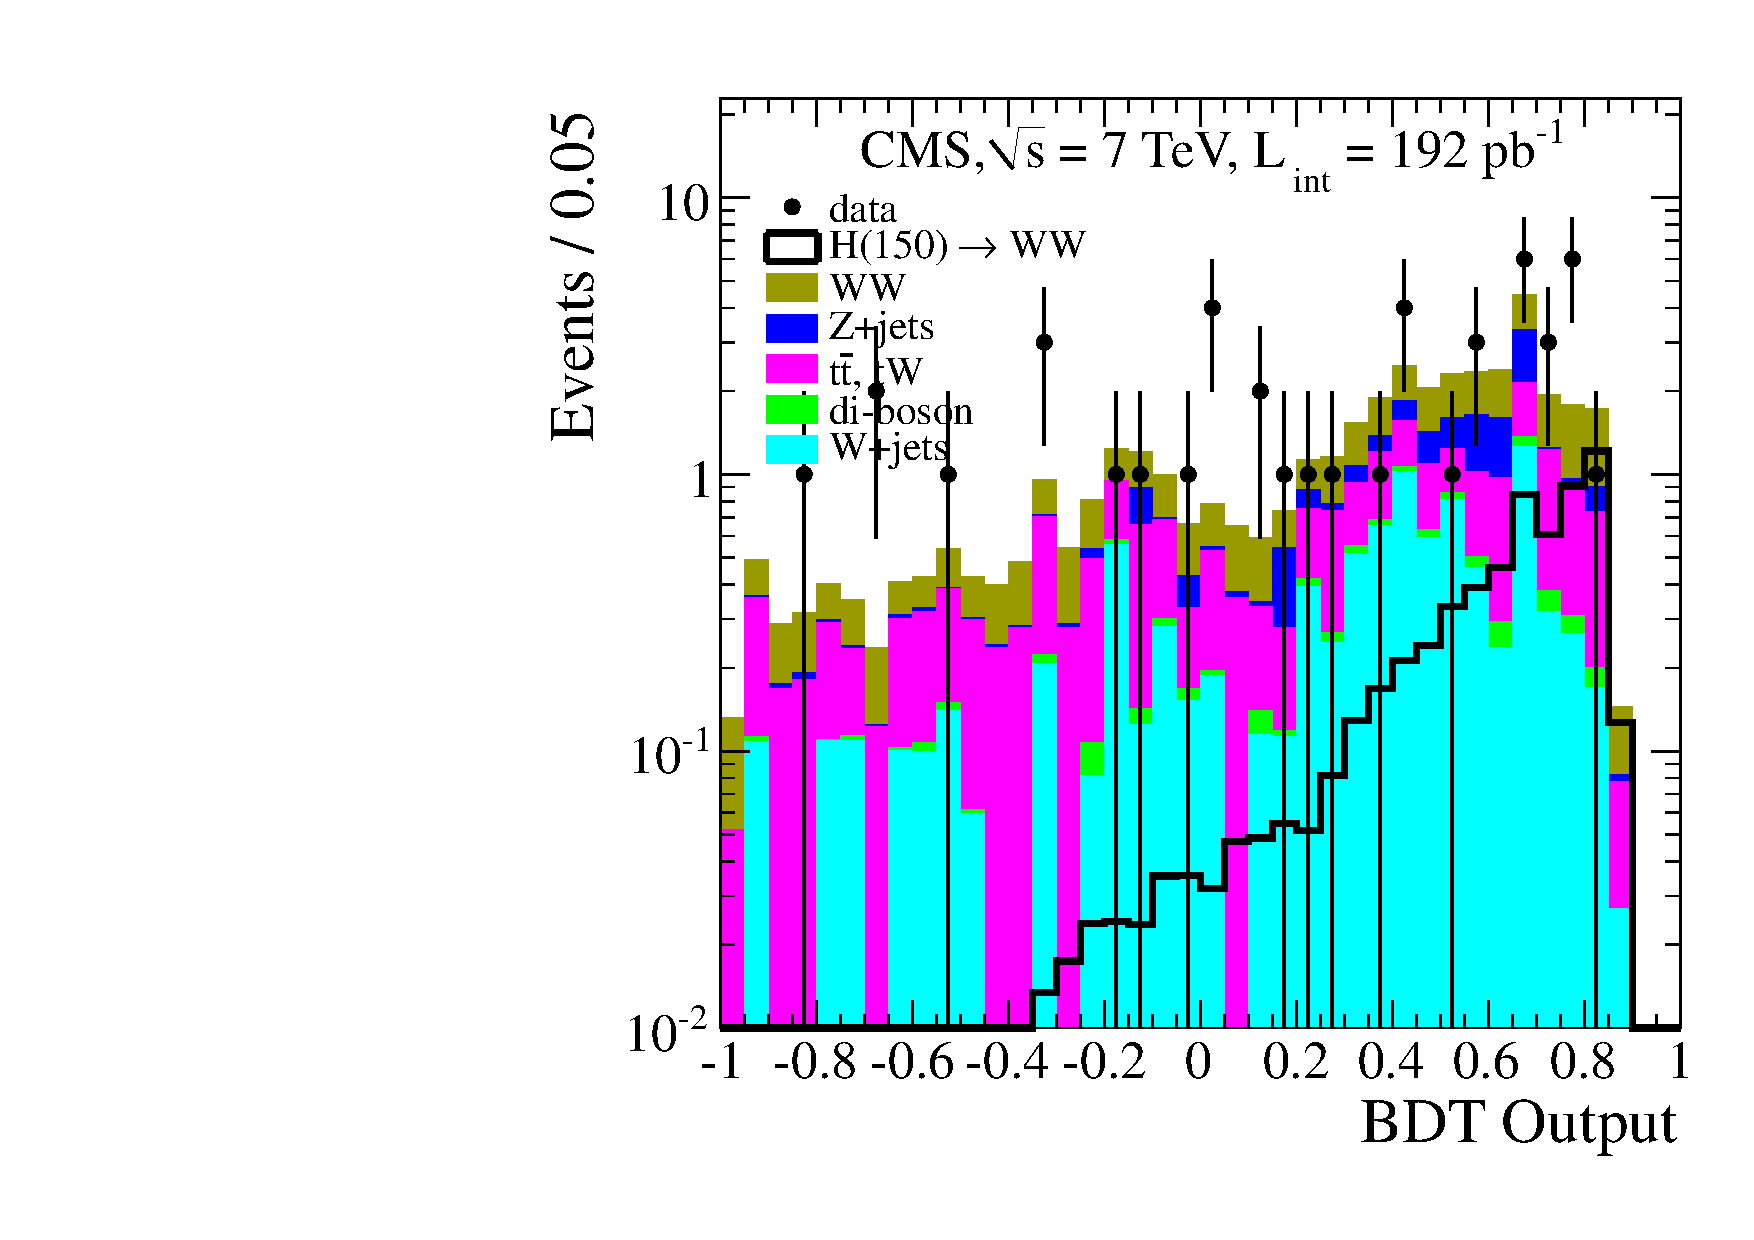
\includegraphics[width=0.49\textwidth,angle=0]{figures/histo_mva_150_1j.pdf}} 
       \caption{Classifier outputs for Higgs signal and background events 
for \mHi=150 $\GeVcc$ in the 0-jet bin (a) and 1-jet bin (b) after the $\WW$ selection. The number 
of events is different on each mass point due to the specific $\mll$ requirement.}
   \label{fig:histo_mva_150}
\end{center}
\end{figure}

\begin{figure}[!ht]
\begin{center}
   \subfigure[]{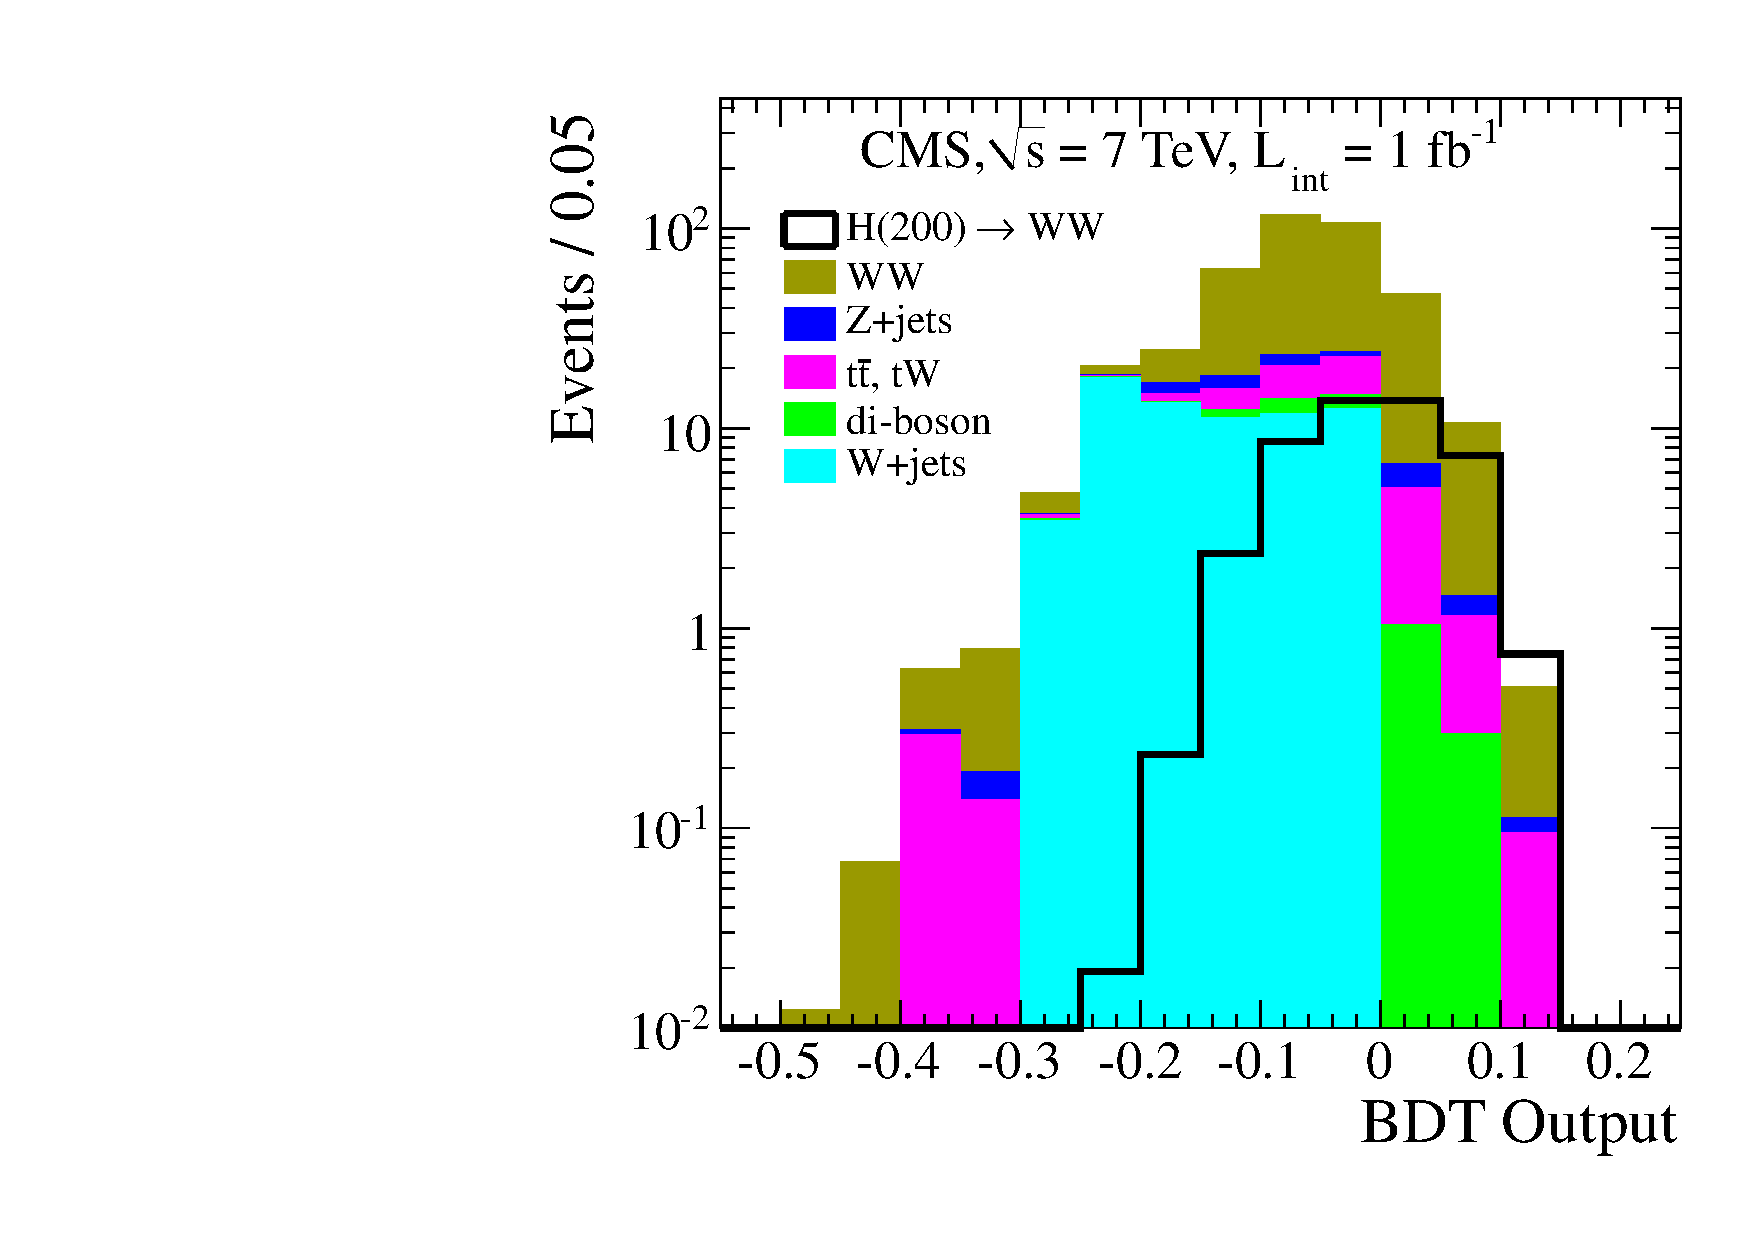
\includegraphics[width=0.49\textwidth,angle=0]{figures/histo_mva_200_0j.pdf}} 
   \subfigure[]{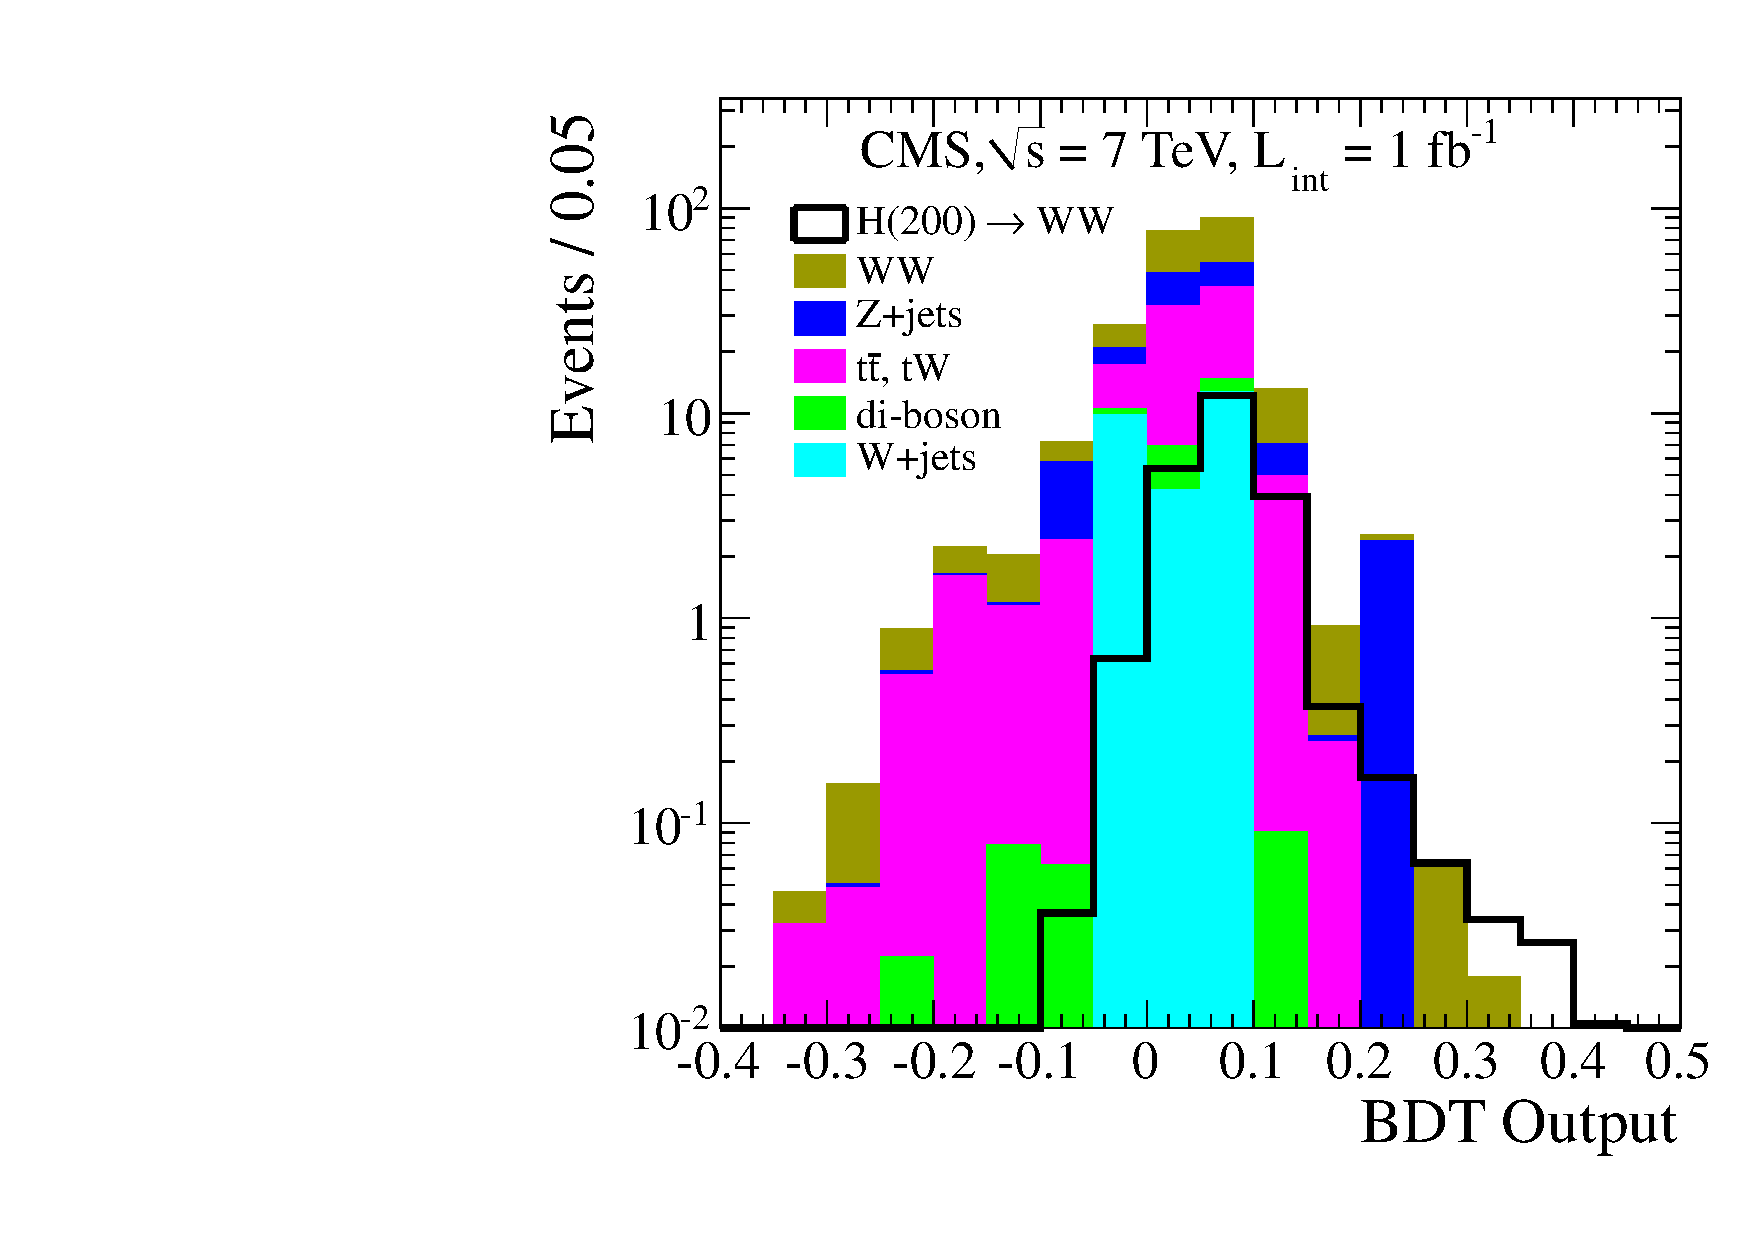
\includegraphics[width=0.49\textwidth,angle=0]{figures/histo_mva_200_1j.pdf}} 
       \caption{Classifier outputs for Higgs signal and background events 
for \mHi=200 $\GeVcc$ in the 0-jet bin (a) and 1-jet bin (b) after the $\WW$ selection. The number 
of events is different on each mass point due to the specific $\mll$ requirement.}
   \label{fig:histo_mva_200}
\end{center}
\end{figure}
\begin{table}[!ht]
  \begin{center}
 {\normalsize
  \begin{tabular} {|c|c|c|c|c|c|}
\hline
  mass    & SM $H\to WW$ & all bkg. & $qq \to \WW$ & $gg \to \WW$ & non-resonant $WZ+ZZ$ \\
  \hline
  \hline
115 &   5.6 $\pm$   0.1 &  49.8 $\pm$   5.7  &  28.7 $\pm$   0.4 &   1.3 $\pm$   0.0 &   0.8 $\pm$   0.1 \\
120 &  10.0 $\pm$   0.1 &  57.9 $\pm$   5.8  &  34.8 $\pm$   0.5 &   1.6 $\pm$   0.0 &   1.1 $\pm$   0.1 \\
130 &  21.4 $\pm$   0.2 &  74.7 $\pm$   6.1  &  47.3 $\pm$   0.5 &   2.4 $\pm$   0.1 &   1.4 $\pm$   0.1 \\
140 &  24.1 $\pm$   0.3 &  48.0 $\pm$   3.8  &  34.4 $\pm$   0.4 &   2.2 $\pm$   0.1 &   0.9 $\pm$   0.1 \\
150 &  25.2 $\pm$   0.3 &  29.9 $\pm$   2.3  &  22.8 $\pm$   0.4 &   1.7 $\pm$   0.0 &   0.5 $\pm$   0.1 \\
160 &  39.0 $\pm$   0.4 &  23.4 $\pm$   2.3  &  16.8 $\pm$   0.3 &   1.7 $\pm$   0.0 &   0.3 $\pm$   0.1 \\
170 &  32.6 $\pm$   0.4 &  20.1 $\pm$   2.1  &  13.7 $\pm$   0.3 &   1.8 $\pm$   0.1 &   0.3 $\pm$   0.0 \\
180 &  22.9 $\pm$   0.3 &  21.8 $\pm$   2.2  &  14.2 $\pm$   0.3 &   2.1 $\pm$   0.1 &   0.3 $\pm$   0.1 \\
190 &  19.1 $\pm$   0.2 &  30.3 $\pm$   1.1  &  21.9 $\pm$   0.4 &   3.0 $\pm$   0.1 &   0.6 $\pm$   0.1 \\
200 &  12.1 $\pm$   0.1 &  25.4 $\pm$   2.2  &  16.6 $\pm$   0.3 &   2.4 $\pm$   0.1 &   0.5 $\pm$   0.1 \\
250 &   6.6 $\pm$   0.1 &  23.9 $\pm$   0.8  &  16.5 $\pm$   0.3 &   1.7 $\pm$   0.0 &   0.4 $\pm$   0.1 \\
300 &   5.9 $\pm$   0.1 &  24.2 $\pm$   0.8  &  17.0 $\pm$   0.3 &   1.4 $\pm$   0.0 &   0.4 $\pm$   0.1 \\
350 &   6.1 $\pm$   0.1 &  20.8 $\pm$   0.7  &  14.5 $\pm$   0.3 &   1.1 $\pm$   0.0 &   0.3 $\pm$   0.0 \\
400 &   5.3 $\pm$   0.1 &  19.4 $\pm$   0.7  &  13.3 $\pm$   0.3 &   1.0 $\pm$   0.0 &   0.3 $\pm$   0.1 \\
450 &   3.1 $\pm$   0.0 &  13.8 $\pm$   0.7  &   9.1 $\pm$   0.2 &   0.8 $\pm$   0.0 &   0.2 $\pm$   0.0 \\
500 &   2.0 $\pm$   0.0 &  11.6 $\pm$   0.6  &   7.5 $\pm$   0.2 &   0.6 $\pm$   0.0 &   0.2 $\pm$   0.0 \\
550 &   1.2 $\pm$   0.0 &   9.3 $\pm$   0.6  &   5.9 $\pm$   0.2 &   0.5 $\pm$   0.0 &   0.1 $\pm$   0.0 \\
600 &   0.7 $\pm$   0.0 &   6.2 $\pm$   0.5  &   4.0 $\pm$   0.2 &   0.3 $\pm$   0.0 &   0.1 $\pm$   0.0 \\
 \hline
  \end{tabular}
  }
 {\normalsize
  \begin{tabular} {|c|c|c|c|}
\hline
  mass    & $\ttbar+tW$ & $\dyll+WZ+ZZ$ & $\Wjets$ \\
  \hline
  \hline
115 &  2.0 $\pm$	0.4 &	2.4 $\pm$   1.2 &  14.6 $\pm$   5.5 \\
120 &  2.4 $\pm$	0.5 &	3.4 $\pm$   1.5 &  14.6 $\pm$   5.5 \\
130 &  3.5 $\pm$	0.6 &	3.5 $\pm$   1.5 &  16.6 $\pm$   5.9 \\
140 &  2.7 $\pm$	0.5 &	1.5 $\pm$   0.8 &   6.2 $\pm$   3.6 \\
150 &  1.6 $\pm$	0.4 &	1.2 $\pm$   0.8 &   2.1 $\pm$   2.1 \\
160 &  1.3 $\pm$	0.4 &	1.1 $\pm$   0.8 &   2.1 $\pm$   2.1 \\
170 &  2.0 $\pm$	0.4 &	0.2 $\pm$   0.0 &   2.1 $\pm$   2.1 \\
180 &  2.7 $\pm$	0.5 &	0.3 $\pm$   0.0 &   2.1 $\pm$   2.1 \\
190 &  3.6 $\pm$	0.6 &	1.3 $\pm$   0.8 &   0.0 $\pm$   0.0 \\
200 &  3.4 $\pm$	0.6 &	0.4 $\pm$   0.0 &   2.1 $\pm$   2.1 \\
250 &  4.9 $\pm$	0.7 &	0.5 $\pm$   0.0 &   0.0 $\pm$   0.0 \\
300 &  5.0 $\pm$	0.7 &	0.4 $\pm$   0.0 &   0.0 $\pm$   0.0 \\
350 &  4.7 $\pm$	0.7 &	0.3 $\pm$   0.0 &   0.0 $\pm$   0.0 \\
400 &  4.5 $\pm$	0.7 &	0.2 $\pm$   0.0 &   0.0 $\pm$   0.0 \\
450 &  3.7 $\pm$	0.6 &	0.2 $\pm$   0.0 &   0.0 $\pm$   0.0 \\
500 &  3.3 $\pm$	0.6 &	0.1 $\pm$   0.0 &   0.0 $\pm$   0.0 \\
550 &  2.6 $\pm$	0.5 &	0.1 $\pm$   0.0 &   0.0 $\pm$   0.0 \\
600 &  1.7 $\pm$	0.4 &	0.1 $\pm$   0.0 &   0.0 $\pm$   0.0 \\
 \hline
  \end{tabular}
  }
  \caption{Expected number of signal and background processes for an 
  integrated luminosity of 1 $\ifb$, after applying the full multivariate analysis 
  selection in the 0-jet bin case. Monte Carlo statistical uncertainties are included.}
   \label{tab:mvasel0j}
  \end{center}
\end{table}

\begin{table}[!ht]
  \begin{center}
 {\normalsize
  \begin{tabular} {|c|c|c|c|c|c|}
\hline
  mass    & SM $H\to WW$ & all bkg. & $qq \to \WW$ & $gg \to \WW$ & non-resonant $WZ+ZZ$ \\
  \hline
  \hline
115 &   1.7 $\pm$   0.0 &  16.5 $\pm$   2.6  &   6.2 $\pm$   0.2 &   0.3 $\pm$   0.0 &   0.6 $\pm$   0.1 \\
120 &   3.3 $\pm$   0.1 &  20.5 $\pm$   2.8  &   8.1 $\pm$   0.2 &   0.4 $\pm$   0.0 &   0.8 $\pm$   0.1 \\
130 &   6.2 $\pm$   0.1 &  19.2 $\pm$   2.4  &   9.3 $\pm$   0.2 &   0.5 $\pm$   0.0 &   0.8 $\pm$   0.1 \\
140 &   9.1 $\pm$   0.1 &  18.9 $\pm$   2.4  &   8.5 $\pm$   0.2 &   0.5 $\pm$   0.0 &   0.6 $\pm$   0.1 \\
150 &  10.1 $\pm$   0.2 &  13.3 $\pm$   1.1  &   6.7 $\pm$   0.2 &   0.4 $\pm$   0.0 &   0.4 $\pm$   0.1 \\
160 &  16.5 $\pm$   0.2 &  13.0 $\pm$   1.1  &   6.5 $\pm$   0.2 &   0.6 $\pm$   0.0 &   0.3 $\pm$   0.1 \\
170 &  13.6 $\pm$   0.2 &  11.4 $\pm$   1.0  &   6.2 $\pm$   0.2 &   0.6 $\pm$   0.0 &   0.2 $\pm$   0.0 \\
180 &   9.2 $\pm$   0.1 &  12.8 $\pm$   1.4  &   6.0 $\pm$   0.2 &   0.5 $\pm$   0.0 &   0.1 $\pm$   0.0 \\
190 &   9.2 $\pm$   0.1 &  21.9 $\pm$   1.5  &  10.9 $\pm$   0.3 &   1.0 $\pm$   0.0 &   0.3 $\pm$   0.1 \\
200 &   6.2 $\pm$   0.1 &  18.6 $\pm$   1.2  &   9.8 $\pm$   0.2 &   0.9 $\pm$   0.0 &   0.2 $\pm$   0.0 \\
250 &   3.8 $\pm$   0.1 &  25.8 $\pm$   2.5  &  10.4 $\pm$   0.2 &   0.4 $\pm$   0.0 &   0.3 $\pm$   0.1 \\
300 &   3.1 $\pm$   0.0 &  20.3 $\pm$   1.4  &   7.8 $\pm$   0.2 &   0.4 $\pm$   0.0 &   0.3 $\pm$   0.1 \\
350 &   4.2 $\pm$   0.0 &  26.5 $\pm$   1.6  &   9.8 $\pm$   0.2 &   0.5 $\pm$   0.0 &   0.4 $\pm$   0.1 \\
400 &   3.6 $\pm$   0.0 &  22.1 $\pm$   1.5  &   8.1 $\pm$   0.2 &   0.4 $\pm$   0.0 &   0.3 $\pm$   0.1 \\
450 &   1.9 $\pm$   0.0 &  12.3 $\pm$   0.9  &   4.6 $\pm$   0.2 &   0.3 $\pm$   0.0 &   0.1 $\pm$   0.0 \\
500 &   1.2 $\pm$   0.0 &   9.5 $\pm$   0.8  &   3.7 $\pm$   0.2 &   0.2 $\pm$   0.0 &   0.1 $\pm$   0.0 \\
550 &   0.8 $\pm$   0.0 &   8.1 $\pm$   0.8  &   3.0 $\pm$   0.1 &   0.2 $\pm$   0.0 &   0.1 $\pm$   0.0 \\
600 &   0.5 $\pm$   0.0 &   5.7 $\pm$   0.7  &   2.0 $\pm$   0.1 &   0.1 $\pm$   0.0 &   0.1 $\pm$   0.0 \\
 \hline
  \end{tabular}
  }
 {\normalsize
  \begin{tabular} {|c|c|c|c|}
\hline
  mass    & $\ttbar+tW$ & $\dyll+WZ+ZZ$ & $\Wjets$  \\
  \hline
  \hline
115 &   4.6 $\pm$   0.7 &   2.7 $\pm$   1.5 &  2.1 $\pm$   2.1 \\
120 &   5.6 $\pm$   0.8 &   3.5 $\pm$   1.7 &  2.1 $\pm$   2.1 \\
130 &   5.5 $\pm$   0.7 &   1.0 $\pm$   0.8 &  2.1 $\pm$   2.1 \\
140 &   6.2 $\pm$   0.8 &   1.0 $\pm$   0.8 &  2.1 $\pm$   2.1 \\
150 &   4.9 $\pm$   0.7 &   1.0 $\pm$   0.8 &  0.0 $\pm$   0.0 \\
160 &   4.6 $\pm$   0.7 &   0.9 $\pm$   0.8 &  0.0 $\pm$   0.0 \\
170 &   3.5 $\pm$   0.6 &   0.9 $\pm$   0.8 &  0.0 $\pm$   0.0 \\
180 &   4.3 $\pm$   0.7 &   1.8 $\pm$   1.2 &  0.0 $\pm$   0.0 \\
190 &   7.9 $\pm$   0.9 &   1.8 $\pm$   1.2 &  0.0 $\pm$   0.0 \\
200 &   6.8 $\pm$   0.8 &   1.0 $\pm$   0.8 &  0.0 $\pm$   0.0 \\
250 &  11.6 $\pm$   1.1 &   1.1 $\pm$   0.8 &  2.1 $\pm$   2.1 \\
300 &  10.8 $\pm$   1.1 &   1.0 $\pm$   0.8 &  0.0 $\pm$   0.0 \\
350 &  14.8 $\pm$   1.3 &   1.0 $\pm$   0.8 &  0.0 $\pm$   0.0 \\
400 &  12.4 $\pm$   1.2 &   0.9 $\pm$   0.8 &  0.0 $\pm$   0.0 \\
450 &   7.3 $\pm$   0.9 &   0.0 $\pm$   0.0 &  0.0 $\pm$   0.0 \\
500 &   5.5 $\pm$   0.8 &   0.0 $\pm$   0.0 &  0.0 $\pm$   0.0 \\
550 &   4.7 $\pm$   0.8 &   0.0 $\pm$   0.0 &  0.0 $\pm$   0.0 \\
600 &   3.6 $\pm$   0.7 &   0.0 $\pm$   0.0 &  0.0 $\pm$   0.0 \\
 \hline
  \end{tabular}
  }
  \caption{Expected number of signal and background processes for an 
  integrated luminosity of 1 $\ifb$, after applying the full multivariate analysis 
  selection in the 1-jet bin case. Monte Carlo statistical uncertainties are included.}
   \label{tab:mvasel1j}
  \end{center}
\end{table}
